\documentclass[usepdftitle=false]{beamer}
% {{{ setup
\usepackage[utf8]{inputenc}
\usepackage{tikz}
\usepackage{pgfplots}
\usepackage{isabelle,isabellesym}

\useoutertheme{infolines}
\setbeamertemplate{headline}[default]
\setbeamertemplate{navigation symbols}{}

\newcommand{\Nat}{\mathbb{N}}
\newcommand{\Real}{\mathbb{R}}

% }}}

% {{{ metadata
\title[Central Limit Theorem]{A formally verified proof of the\\ Central Limit Theorem\\(preliminary report)}
\author[Avigad (CMU), \underline{H\"olzl (TUM)}, Serafin (CMU)]{%
  \begin{tabular}[t]{@{}c@{}}
    Jeremy Avigad
    \\[2ex]
    \usebeamerfont{institute}
    Carnegie Mellon University
  \end{tabular}
  \quad
  \and
  \quad
  \begin{tabular}[t]{@{}c@{}}
    \underline{Johannes H\"olzl}
    \\[2ex]
    \usebeamerfont{institute}
    TU M\"unchen
  \end{tabular}
  \and
  \quad
  \begin{tabular}[t]{@{}c@{}}
    Luke Serafin
    \\[2ex]
    \usebeamerfont{institute}
    Carnegie Mellon University
  \end{tabular}
  \vspace{-3ex}
}
\date[Isabelle Workshop 2014]{\small Isabelle Workshop 2014}

% PDF settings
\hypersetup{%
  pdftitle={A formally verified proof of the\\ Central Limit Theorem\\(preliminary report)},
  pdfauthor={Jeremy Avigad, Johannes H\"olzl, and Luke Serafin}%
}
% }}}

\begin{document}

\begingroup % {{{ titlepage
\setbeamertemplate{footline}{} % supress info footline on title page
\begin{frame}
  \maketitle
\end{frame}
\endgroup % }}}

\begin{frame}{Motivation} % {{{


\begin{center}
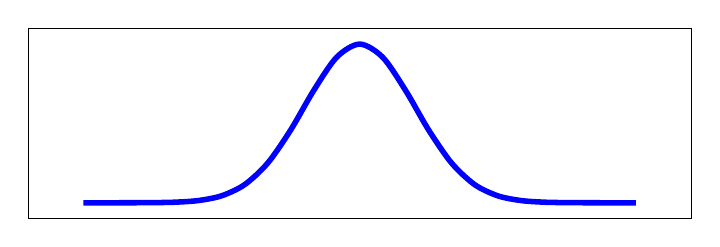
\begin{tikzpicture}
  \begin{axis}[width=10cm, height=4cm, ticks = none]
    
    \addplot[color=blue, line width = 2pt, smooth] {1 / sqrt (2 * pi) * exp(-(x ^ 2) / 2)};
    
  \end{axis}
\end{tikzpicture}
\end{center}
\begin{center} Why is the normal distribution interesting? \end{center}

\begin{center}
\Large
  The \emph{Central Limit Theorem} tells us: \\
  it is the average of infinitely many errors.
\end{center}


\end{frame} % }}}

\begin{frame}{Central Limit Theorem -- informal} % {{{
\begin{center}
\begin{tikzpicture}
  \begin{axis}[width=10cm,
      xmin = -3,
      xmax = 3,
      ymin = 0,
      ymax = 0.5,
      ticks = none,
      ybar, bar shift = {0cm},
      bar width = 2pt]
    
    \only<5,6>{\addplot[fill=red!10] table {binomial-512.dat};}
    \only<4>{\addplot[fill=red!30] table {binomial-128.dat};}
    \only<3>{\addplot[fill=red!50] table {binomial-32.dat};}
    \only<2>{\addplot[fill=red!70] table {binomial-8.dat};}
    \only<1>{\addplot[fill=red!90] table {binomial-2.dat};}
    
    \only<6>{\addplot[color=blue, line width = 2pt, smooth] {1 / sqrt (2 * pi) * exp(-(x ^ 2) / 2)};}
    
  \end{axis}
\end{tikzpicture}
\end{center}
\end{frame} % }}}

\begin{frame}{Central Limit Theorem -- formal} % {{{

\begin{itemize}

\item Sequence of random variables: $X : \Nat \to \Omega \to \Real$

\item They are i.i.d.\ (independent and identically distributed)

\item Expectation: $\mathbb{E}[X_i] = 0$ and variance: $\mathbb{V}[X_i] = \sigma^2$ (for all $i$)

\end{itemize}

\[ \frac{1}{\sqrt{n \sigma^2}} \sum_{i < n} X_i \xrightarrow{\quad n \to \infty \quad} \mathcal{N}(0, 1) \]

\end{frame} % }}}

\begin{frame}{Central Limit Theorem -- in Isabelle/HOL} % {{{

\begin{isabellebody}
\isacommand{theorem}\isamarkupfalse%
\ {\isacharparenleft}\,\isakeyword{in}\ prob{\isacharunderscore}space{\isacharparenright}\ central{\isacharunderscore}limit{\isacharunderscore}theorem{\isacharcolon}\isanewline
\ \ \isakeyword{fixes}\ \isanewline
\ \ \ \ X\ {\isacharcolon}{\isacharcolon}\ {\isachardoublequoteopen}nat\ {\isasymRightarrow}\ {\isacharprime}a\ {\isasymRightarrow}\ real{\isachardoublequoteclose}\ \isakeyword{and}\isanewline
\ \ \ \ D\ {\isacharcolon}{\isacharcolon}\ {\isachardoublequoteopen}real\ measure{\isachardoublequoteclose}\ \isakeyword{and}\isanewline
\ \ \ \ {\isasymsigma}\ {\isacharcolon}{\isacharcolon}\ real\isanewline
\pause
\ \ \isakeyword{assumes}\isanewline
\ \ \ \ {\isachardoublequoteopen}indep{\isacharunderscore}vars\ {\isacharparenleft}{\isasymlambda}i{\isachardot}\ borel{\isacharparenright}\ X\ UNIV{\isachardoublequoteclose}\ \isakeyword{and}\isanewline
\ \ \ \ {\isachardoublequoteopen}{\isasymAnd}n{\isachardot}\ distr\ M\ borel\ {\isacharparenleft}X\ n{\isacharparenright}\ {\isacharequal}\ D{\isachardoublequoteclose}
\pause\ \isakeyword{and}\isanewline
\ \ \ \ {\isachardoublequoteopen}{\isasymAnd}n{\isachardot}\ integrable\ M\ {\isacharparenleft}X\ n{\isacharparenright}{\isachardoublequoteclose}\ \isakeyword{and}\isanewline
\ \ \ \ {\isachardoublequoteopen}{\isasymAnd}n{\isachardot}\ expectation\ {\isacharparenleft}X\ n{\isacharparenright}\ {\isacharequal}\ {\isadigit{0}}{\isachardoublequoteclose}
\pause\ \isakeyword{and}\isanewline
\ \ \ \ {\isachardoublequoteopen}{\isasymsigma}\ {\isachargreater}\ {\isadigit{0}}{\isachardoublequoteclose}\ \isakeyword{and}\isanewline
\ \ \ \ {\isachardoublequoteopen}{\isasymAnd}n{\isachardot}\ integrable\ M\ {\isacharparenleft}{\isasymlambda}x{\isachardot}\ {\isacharparenleft}X\ n\ x{\isacharparenright}\isactrlsup {\isadigit{2}}{\isacharparenright}{\isachardoublequoteclose}\ \isakeyword{and}\isanewline
\ \ \ \ {\isachardoublequoteopen}{\isasymAnd}n{\isachardot}\ variance\ {\isacharparenleft}X\ n{\isacharparenright}\ {\isacharequal}\ {\isasymsigma}\isactrlsup {\isadigit{2}}{\isachardoublequoteclose}\isanewline
\ \ \isakeyword{shows}\isanewline
\ \ \ \ {\isachardoublequoteopen}weak{\isacharunderscore}conv{\isacharunderscore}m\ \isanewline
\ \ \ \ \ \ \ \ {\isacharparenleft}{\isasymlambda}n{\isachardot}\ distr\ M\ borel\ {\isacharparenleft}{\isasymlambda}x{\isachardot}\ {\isasymSum}i{\isacharless}n{\isachardot}\ X\ i\ x\ {\isacharslash}\ sqrt\ {\isacharparenleft}n\ {\isacharasterisk}\ {\isasymsigma}\isactrlsup {\isadigit{2}}{\isacharparenright}{\isacharparenright}{\isacharparenright}\isanewline
\ \ \ \ \ \ \ \ {\isacharparenleft}density\ lborel\ standard{\isacharunderscore}normal{\isacharunderscore}density{\isacharparenright}{\isachardoublequoteclose}
\end{isabellebody}

\end{frame} % }}}

\begin{frame}{Concepts} % {{{
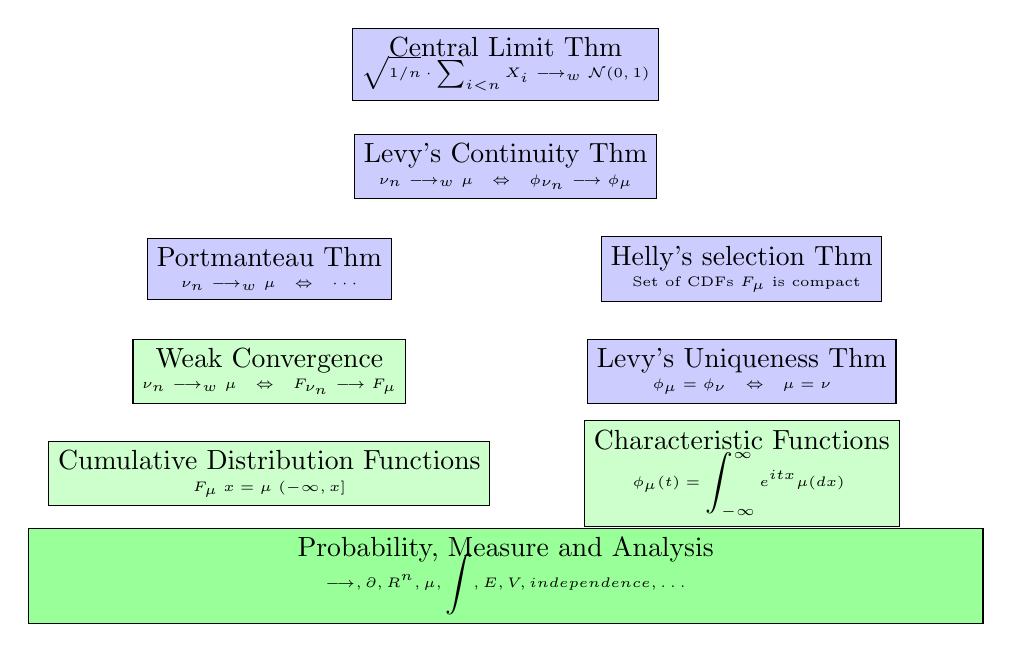
\begin{tikzpicture}[align=center, yscale=1.3,
    thm/.style={draw, fill=blue!20},
    thy/.style={draw, fill=green!20}]

  \node[draw, fill=green!40, minimum width=\textwidth] at ( 0, 0)
    { Probability, Measure and Analysis \\[-1ex] {\tiny $
      \displaystyle \longrightarrow, \partial, \mathbb{R}^n, \mu, \int, \mathbb{E}, \mathbb{V}, \text{independence}, \dots $} } ;
\pause      
  \node[thy] at (-3, 1) { Cumulative Distribution Functions \\[-1ex] {\tiny $
    F_\mu\;x = \mu~(-\infty, x] $} } ;

\pause

  \node[thy] at (-3, 2) { Weak Convergence \\[-1ex] {\tiny $
    \nu_n ~ {\longrightarrow}_w ~ \mu ~~\Leftrightarrow~~ F_{\nu_n} \longrightarrow F_\mu $} } ;

\pause

  \node[thm] at (-3, 3) { Portmanteau Thm \\[-1ex] {\tiny $
    \nu_n ~ {\longrightarrow}_w ~ \mu ~~ \Leftrightarrow ~~ \cdots $} } ;

\pause

  \node[thy] at ( 3, 1) { Characteristic Functions \\ {\tiny $\displaystyle
    \phi_\mu(t) = \int_{-\infty}^{\infty} e^{itx} \mu(dx) $ } } ;

  \node[thm] at ( 3, 2) { Levy's Uniqueness Thm \\[-1ex] {\tiny $
    \phi_\mu = \phi_\nu ~~ \Leftrightarrow ~~ \mu = \nu $ }} ;

\pause

  \node[thm] at ( 3, 3) { Helly's selection Thm \\[-1ex] { \tiny
    Set of CDFs $F_\mu$ is compact }} ;

  \node[thm] at ( 0, 4) { Levy's Continuity Thm \\[-1ex] {\tiny $
    \nu_n~{\longrightarrow}_w~\mu ~~\Leftrightarrow~~ \phi_{\nu_n} \longrightarrow \phi_\mu $} } ;

\pause

  \node[thm] at ( 0, 5) { Central Limit Thm \\[-1ex] {\tiny $
    \sqrt{1/n} \cdot \sum_{i<n} X_i ~ {\longrightarrow}_w ~ \mathcal{N}(0,1) $} } ;

\end{tikzpicture}
\end{frame} % }}}

\begin{frame}{Weak convergence of measures} % {{{

\begin{definition}[Cumulative Distribution Function]%
\vspace{-1ex}
\begin{center}%
$ F_\mu~x := \mu~(-\infty, x] $
\end{center}
\end{definition}

\begin{definition}[Weak convergence]
\begin{center} 
$ \begin{array}{l} \nu_n ~{\longrightarrow}_w~ \mu :\Leftrightarrow \\
\qquad
  (\forall t.~ F_\mu~\text{continuous at}~ t \implies
       (F_{\nu\,n}~t) \longrightarrow F_\mu~t)
  \end{array} $
\end{center}
{\small (In Isabelle/HOL written as: \texttt{weak{\_}conv{\_}m})}
\end{definition}

\begin{theorem}[Portmanteau Theorem]
Equivalent characterizations of $\nu_n ~{\longrightarrow}_w~ \mu$:
\begin{itemize}
 \item $\int f \; d\nu_n~{\longrightarrow}_w~\int f \; d\mu$ ~~ for every bounded, continuous $f$
 \item $\nu_n~A ~ {\longrightarrow}_w ~ \mu_n~A$ ~~ for all Borel sets $A$, with $\mu(\partial A) = 0$
\end{itemize}
\end{theorem}

\end{frame} % }}}


\begin{frame}{Characteristic functions} % {{{

\begin{definition}[Characteristic functions]%
\vspace{-1em}
\begin{center} $ \displaystyle \phi_\mu~t = \int_{-\infty}^{\infty} e^{itx} \mu(dx) $ \end{center}
\end{definition}

\begin{theorem}[Levy Uniqueness Theorem]
\vspace{-1em}
\begin{center} $ \phi_{\mu_1} = \phi_{\mu_2} \Leftrightarrow \mu_1 = \mu_2 $ \end{center} 
\end{theorem}

\begin{theorem}[Levy Continuity Theorem]
\vspace{-1em}
\begin{center} $ \nu_n ~{\longrightarrow}_w~ \mu \Leftrightarrow
  (\forall t.\ \phi_{\nu_n}~t \xrightarrow{n \to \infty} \phi_\mu~t) $ \end{center}
\end{theorem}

Also the characteristic function of the std. normal distribution:
\[ \phi_{\mathcal{N}(0, 1)}~t = e^{-t^2/2}\]

\end{frame} % }}}

\begin{frame}{Central Limit Theorem -- the proof} % {{{
\begin{itemize}

  \item Show $\phi_{\sqrt{1/n} \sum_{i < n} X_i}$ approaches $\phi_{\mathcal{N}(0, 1)}$
    
  \item We have $\phi_{\mathcal{N}(0, 1)}~t = e^{-t^2/2}$
  
  \item We have $\phi_{\sum_{i < n} X_i}~t = (\phi_D~t)^n$ 
  
  \item Finishing using power series approximation of the exponential function
  
  \item Size of the final CLT proof: 120 lines of theory
\end{itemize}
\end{frame} % }}}

\begin{frame}{Summary} % {{{
\begin{itemize}
\item Current size: $\approx 6,250$ lines of thy
\item Paper mentions $\approx 13,000$ lines\\
  some clean up some stuff moved to the repository
\begin{itemize}

\item Generalized Lebesgue integration to Bochner integration: \\
  $\int {f}\; d\!\mu :: \mathbb{R}$ to $\int {f}\; d\!\mu :: \mathbb{R}^n$ and separable $\mathbb{R}$-normed vector spaces \\
  (unifies $\mathbb{R}$ and $\mathbb{C}$)

\item Definition of the Lebesgue-Stieltjes measure: \\ 
  $\mathcal{L}_F~[a, b] = F~b - F~a$
\end{itemize}

\item CLT fundamental to contemporary probability theory\\
  but also the necessary machinery!

\end{itemize}
\end{frame} % }}}


\end{document}
